\section{Hiện thực Database}
    \subsection{ER Diagram}
    Dựa vào Use-case Diagram kèm theo các mô tả cho từng use-case ở phần 2. Xác định được các thực thể và mối quan hệ cho Database như sau:
        \begin{itemize}
            \item Thực thể: \textbf{User}, \textbf{account}, \textbf{admin}, \textbf{food}, \textbf{ingredient}.
            \item Mối quan hệ: User-\textbf{review}-food, User-\textbf{pick}-food, food-\textbf{contain}-ingredient, admin-\textbf{edited}-food, account-\textbf{belongto}-admin, admin-\textbf{manage}-account.
        \end{itemize}
        \begin{figure}[h]
            \centering
            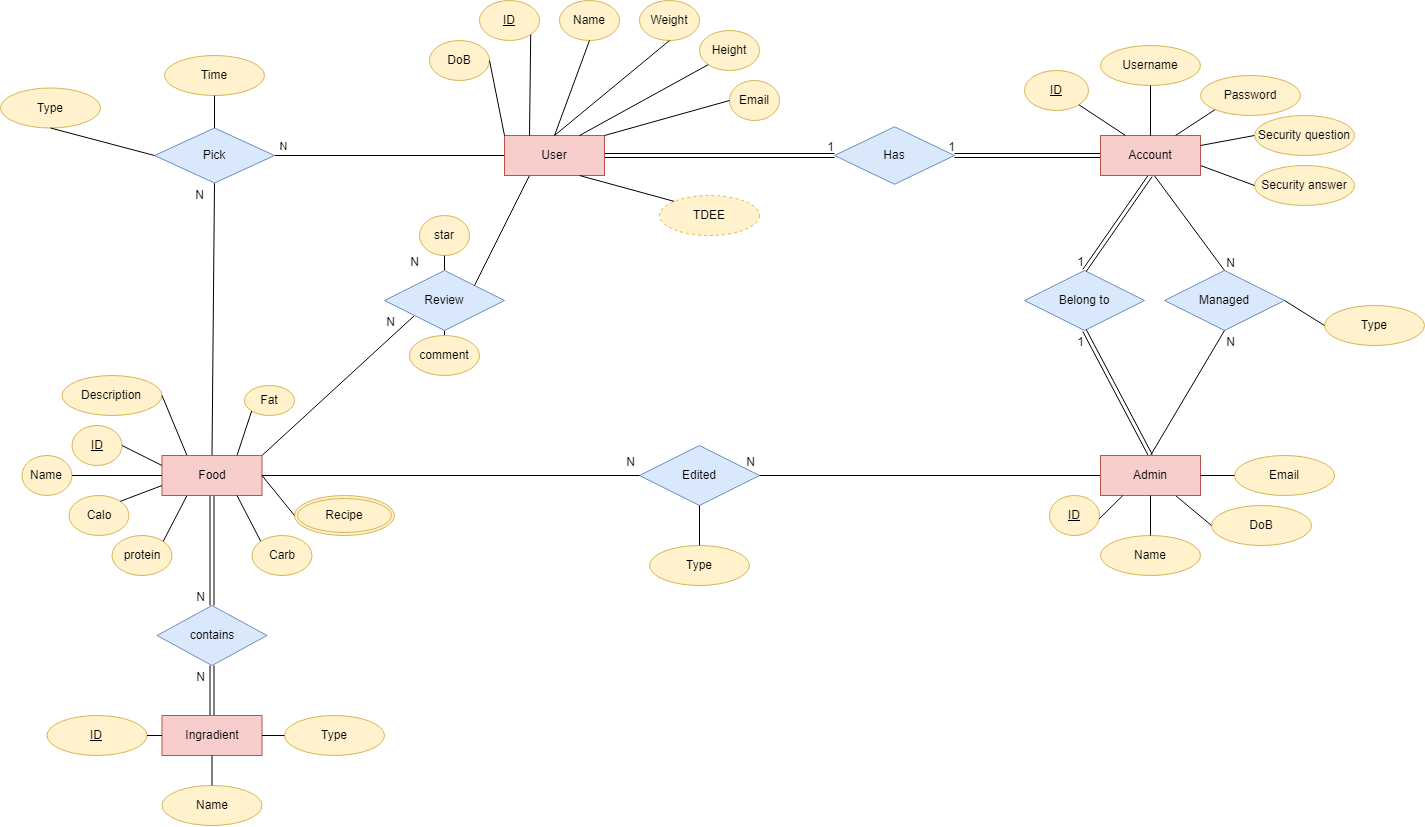
\includegraphics[width=0.99\linewidth]{images/backendDB/Foody_DB-ERD.drawio.png}
            \caption{ER Diagram of FOODY}
        \end{figure}
    \textbf{Link ảnh:} https://drive.google.com/file/d/1lA7-aU0gCllVa-p-Sp3iiUXmH4snUN0m/view?usp=sharing
    \newpage
    \subsection{Mapping}
        \begin{figure}[h]
            \centering
            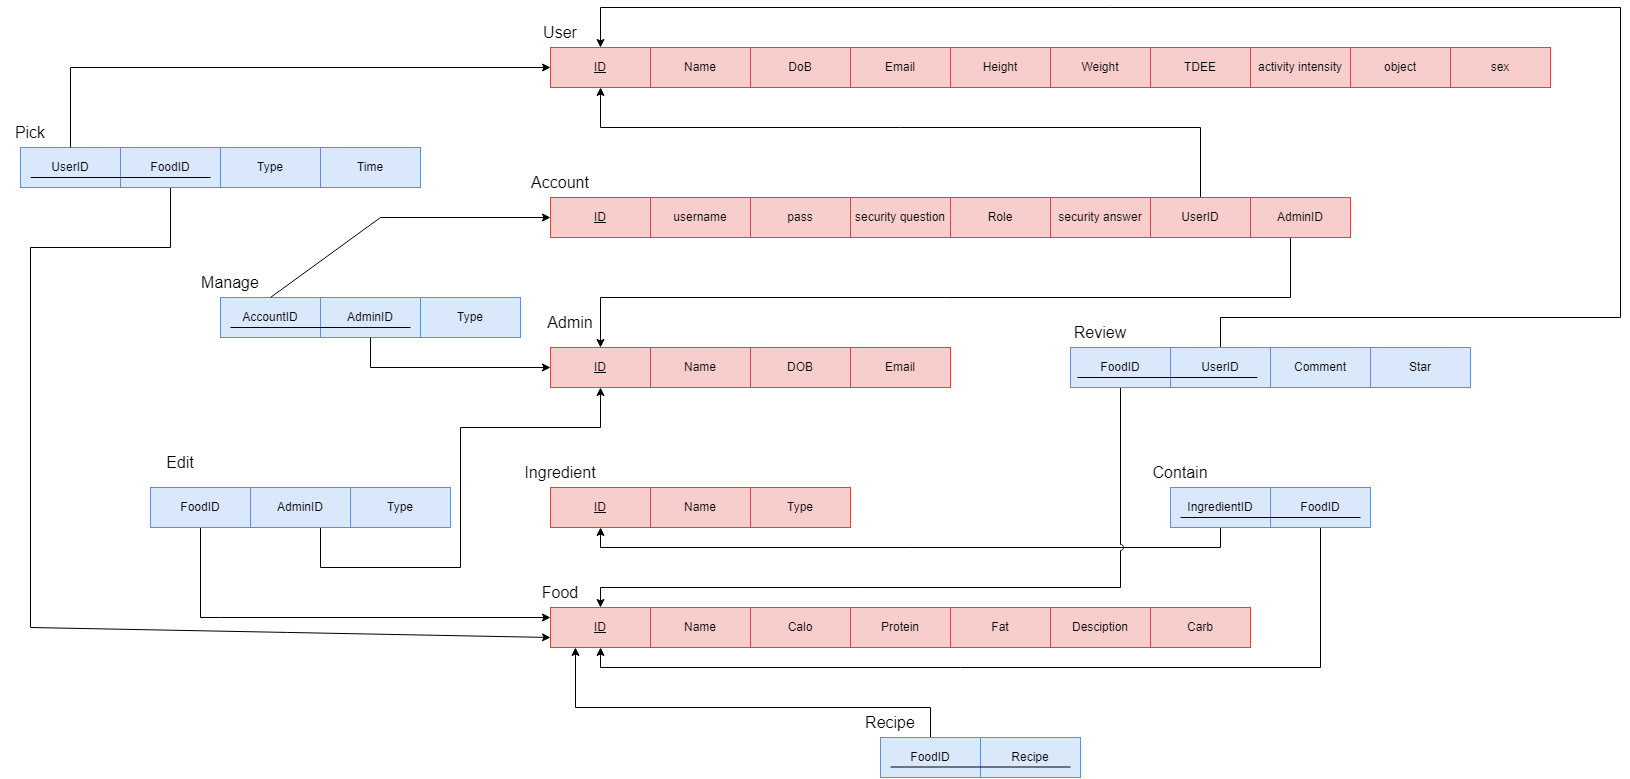
\includegraphics[width=0.99\linewidth]{images/backendDB/Foody_DB-Mapping.drawio.png}
            \caption{Mapping of FOODY}
        \end{figure}
        \textbf{Link ảnh:} https://drive.google.com/file/d/1NyA6kv1SKYCjilm013Aqxx2CA7a8xhSQ/view?usp=sharing
    \newpage
    \subsection{Tables in Mysql}
    Dựa vào thiết kết ý niệm và thiết kế luận lý ở ERD và Mapping ở trên, có thể hiện thực trong Mysql và có kết quả như sau:
        \begin{figure}[h]
            \centering
            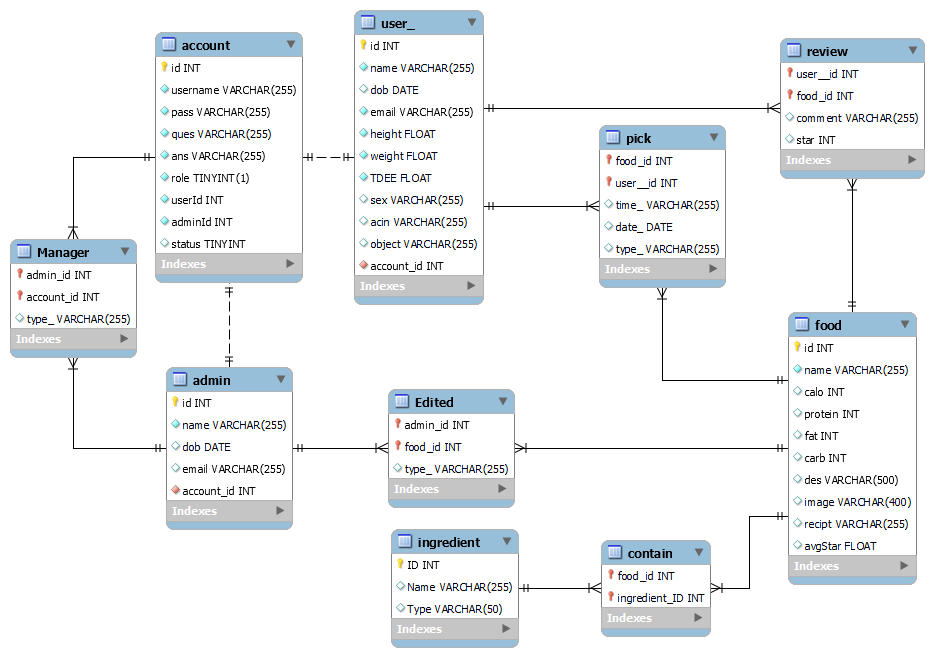
\includegraphics[width=0.99\linewidth]{images/backendDB/sqltable.png}
            \caption{In Mysql}
        \end{figure}
        \textbf{Link ảnh:} https://drive.google.com/file/d/1-6Bw8UxXbeNI\_D4qqNOI5LfYTKBnHXyI/view?usp=sharing